\documentclass[12pt, a4paper, oneside]{article}
\usepackage[utf8]{inputenc}
\usepackage{fancyhdr}
\usepackage{graphicx}
\usepackage{caption}
\usepackage{tikz}
\usetikzlibrary{calc}
\newcommand\HRule{\rule{\textwidth}{1pt}}
\usepackage[parfill]{parskip}
\usepackage[acronym]{glossaries}
\usepackage{url}
\usepackage[round]{natbib}
\usepackage[scientific-notation=true]{siunitx}
\setlength{\arrayrulewidth}{0.4mm}
\setlength{\tabcolsep}{4pt}
\renewcommand{\arraystretch}{1.5}
\usepackage{tabularx, makecell, booktabs}
\renewcommand{\cellalign}{lc}
\renewcommand{\theadalign}{lc}
\renewcommand{\theadfont}{\normalsize\bfseries}

\usepackage{setspace}
\onehalfspacing
\makeglossaries

\bibliographystyle{agsm}

\setlength{\headheight}{15pt}

\graphicspath{ {./images/} }

\usepackage{courier} %% Sets font for listing as Courier.
\usepackage{listings, xcolor}
\lstset{
tabsize = 4, %% set tab space width
showstringspaces = false, %% prevent space marking in strings, string is defined as the text that is generally printed directly to the console
numbers = left, %% display line numbers on the left
commentstyle = \color{green}, %% set comment color
keywordstyle = \color{blue}, %% set keyword color
stringstyle = \color{red}, %% set string color
rulecolor = \color{black}, %% set frame color to avoid being affected by text color
basicstyle = \small \ttfamily , %% set listing font and size
breaklines = true, %% enable line breaking
numberstyle = \tiny,
}

\pagestyle{fancy}
\fancyhf{}
\rhead{MSc Enterprise Software Systems}
\rfoot{\thepage}

\title{\textbf{Analysis and Evaluation of Kubernetes based Multi-Cluster Service Discovery Service Mesh Solutions}}
\author{Robert O'Brien\\[0.5cm]{Supervisor: Dr. Siobhan  Drohan}\\[0.5cm]{MSc Enterprise Software Systems}}
\date{January 2021}

\newacronym{msa}{MSA}{Microservice Architecture}
\newacronym{k8s}{K8s}{Kubernetes}
\newacronym{kep}{KEP}{Kubernetes Enhancement Protocol}
\newacronym{sd}{SD}{Service Discovery}
\newacronym{sm}{SM}{Service Mesh}

\begin{document}
\begin{titlepage}
	\maketitle
	\thispagestyle{empty}
	
\begin{tikzpicture}[remember picture, overlay]
		\draw[line width = 1pt] ($(current page.north west) + (1in,-1in)$) rectangle ($(current page.south east) + (-1in,1in)$);
	\end{tikzpicture}
	\newpage
					
\end{titlepage}
\tableofcontents
\newpage

\listoffigures
\listoftables
\newpage

\printglossary[type=\acronymtype]
\newpage

\section*{Plagiarism Declaration}
I confirm that this assignment is my work, that it is not copied from any other person’s work (whether published or unpublished). I am aware that any user of material from other works (including paraphrase) without citation will be treated as plagiarism. The sources of any material quoted or referenced are provided and acknowledged.

Robert O’Brien
\newpage
\section{Introduction}
\acrshort{msa}s (MSA) have seen a rise in popularity due to containerised orchestration platforms such as \acrshort{k8s} (K8s). They facilitate creating smaller, loosely coupled services that can be released independently of each other, accelerating development cycles and increasing flexibility. Container Orchestration Platforms such as the \acrshort{k8s} manage and orchestrate containerised applications, which are application packaged into individual, lightweight runtime environments containing everything needed to run a microservice. Load Balancing, automated scaling, and service discovery (SD) are just some of the features provided by container orchestration platforms. 

The advantages offered by container orchestration platforms are not without cost. The greater the number of services running in a distributed system, the more complex it becomes. Microservices are often dependent on each other and need to communicate to work as part of a more extensive, coherent system. \acrshort{k8s} clusters are traditionally single cluster setups, but as many companies and organisations move their microservice-based applications to container orchestration platforms, multi-cluster designs are becoming more common. \acrshort{sd} is an intrinsic part of modern MSAs and not just container orchestration platforms. Interservice communication within modern MSAs have had to evolve to accommodate the ever-growing number of services that make up today’s applications. Complexity is hard to scale, even more so when dependent services to span multiple clusters. \acrlong{sm}es (\acrshort{sm}) help reduce this complexity by controlling the communication within \acrshort{msa}s.   

This study analyses how current multi-cluster \acrshort{sd} \acrshort{sm} solutions solve this problem, as many take a novel approach. A variety of solutions will then be evaluated using the following categories: configuration complexity, health-checks, load balancing and security.
\newpage

\section{Background}
\subsection{Multi-Cluster}
A single \acrshort{k8s} instance is termed a cluster. The term multi-cluster refers to two or more independent \acrshort{k8s} clusters used to form a larger connected system of clusters that communicate over a network. \acrshort{k8s} multi-cluster setups are becoming more popular. Support for multiple cloud providers and hybrid environments has increased, primarily to allow for increased isolation for specific services and require high performance and fault tolerance levels. One of the drawbacks of multiple \acrshort{k8s} clusters is the absence of a feature allowing services in different clusters to discover each other over a network. As multi-cluster \acrshort{sd} is not a native \acrshort{k8s} feature, many third-party solutions have stepped in to solve this problem using various architectural approaches and discovery mechanisms. Figure 1 below shows a basic multi-cluster federation architecture:
\begin{center}
	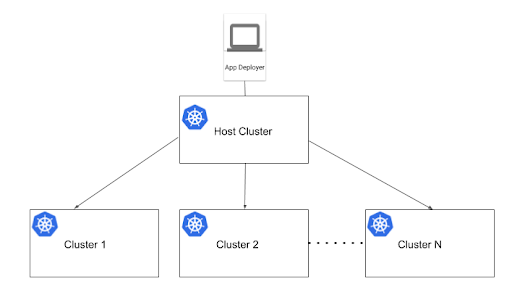
\includegraphics[scale=0.7]{images/cluster-federation.png}
	\begin{figure}[hp]
		\caption[Example of a multi-cluster federation architecture]{Example of a multi-cluster federation architecture \citep{multicluster}}
	\end{figure}
\end{center}

\subsection{Service Discovery}
\acrshort{k8s} is the process by which a service exposed from a cluster is made available for DNS requests from clients (Suryanarayanan, 2020). The clients in a multi-cluster setup can consist of services located on different clusters, a single service deployed on multiple clusters or external services outside of a cluster that consumes the service. Microservices within a \acrshort{k8s} cluster are deployed in what are known as pods. Each pod is assigned an internal IP address, which allows communication between pods within the same cluster. Still, due to a pods’ ephemeral nature (they can be created, scaled, destroyed and updated during their lifecycle), a pod’s IP address is a dynamic property. To account for this, \acrshort{k8s} uses an additional resource known as a service. A service is an abstraction above a grouping of pods that receives all networking requests, and load balances the requests between the pods associated with the service. As the services’ IP address is static (unless configured otherwise), the cluster’s multiple services can communicate. While this is sufficient for a single cluster setup, clusters in a multi-cluster setup have no way of knowing what services are exposed outside its boundary. Figure 2 below displays an example of how the Submariners Lighthouse project facilitates cross-cluster \acrshort{sd}:

\begin{center}
	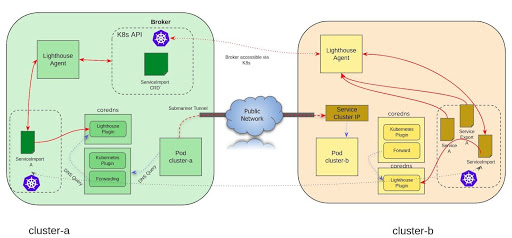
\includegraphics[scale=0.7]{images/service-discovery.jpg}
	\begin{figure}[hp]
		\caption[Multi-cluster service discovery architecture with Submariner and Lighthouse]{Multi-cluster service discovery architecture with Submariner and Lighthouse \citep{submariner}}
	\end{figure}
\end{center}

\subsection{Service Mesh}
A service mesh (SM) is a configurable, low‑latency infrastructure layer designed to handle a high volume of network‑based interprocess communication among application infrastructure services using application programming interfaces (Smith and Garrett, 2020). The most common SM design pattern is the sidecar design pattern. In this pattern, a proxy service (commonly known as a sidecar) is deployed alongside each service to act as a gateway for requests bound for the service. As all networking requests travel through the sidecar proxy, networking concerns such as authentication, observability, routing, and security are handled by the acrshort{sm}, allowing for a more resilient networking design. Many of today’s \acrshort{sm}s offer multi-cluster SD. Figure 3 below displays an example of the sidecar design pattern within a SM:

\begin{center}
	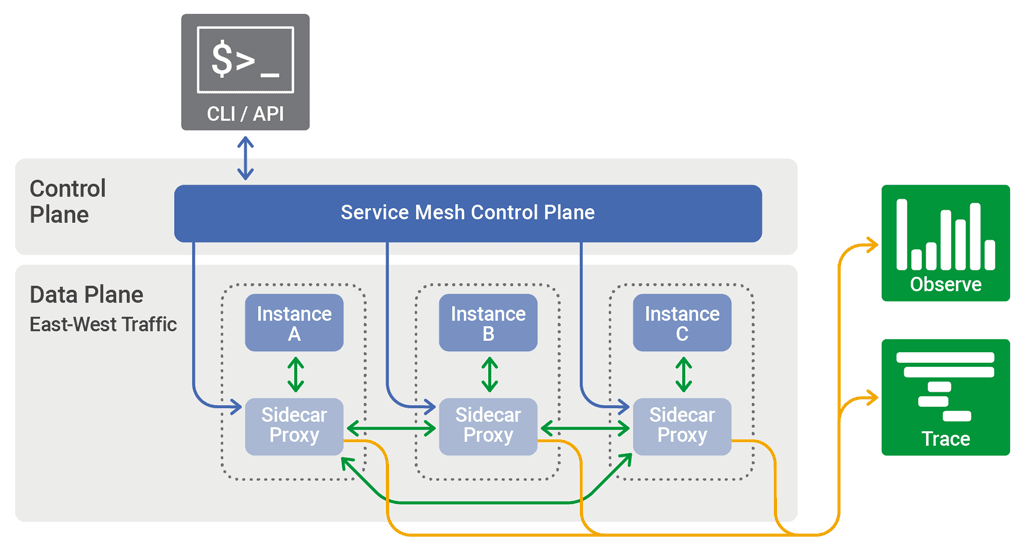
\includegraphics[scale=0.4]{images/service-mesh-architecture.png}
	\begin{figure}[hp]
		\caption[Generic service mesh topology]{Generic service mesh topology \citep{sm_image}}
	\end{figure}
\end{center}


\newpage

\section{Scope}
This study's primary goal is to analyse multi-cluster \acrshort{sm} \acrshort{sd} solutions to determine what design architectures and discovery mechanism each solution employs to overcome the challenges associated with multi-cluster \acrshort{sd}. Each solution will then be evaluated under the following categories: configuration complexity, health-checks, load balancing and security. The evaluation process will use a Proof of Concept environment consisting of two or more \acrshort{k8s} clusters to simulate a multi-cluster setup. The solutions under evaluation study must be open-source and in a mature state of development. Hybrid or multi-cloud \acrshort{k8s} configurations are outside of the scope of the study. Time permitting, the study will be extended to compare the \acrshort{sd} architecture of the current solutions with the proposed solution in the \acrshort{k8s} Enhancement Proposal (\acrshort{kep}) related to this problem.

\section{Research Problem}
There is currently no standard way to connect or even think about \acrshort{k8s} services beyond the cluster boundary. Still, we increasingly see users deploy applications across multiple clusters designed to work in concert \citep{kep}. While many third-party \acrshort{sm} solutions exist to alleviate this problem, the design approaches and method each takes differs significantly. It is not always obvious which solution is the most suitable for each specific use case or performs best in specific areas. This study will analyse each solution’s design architecture and implementation approach before evaluating each under four chosen categories which make up important decision factors associated with \acrshort{sd}: configuration complexity, service level health-checks, service level load balancing and inter-service security. Native support in the \acrshort{k8s} community for multi-cluster \acrshort{sd} is scheduled in the form of a \acrshort{k8s} \acrshort{kep}. As of writing, the \acrshort{kep} is in an Alpha development stage and no target \acrshort{k8s} release version or time frame exists as to when this feature will be made generally available.
\newpage

\section{Research Questions}
\begin{enumerate}
	\item What design architectures and discovery mechanisms do current open-source Service Mesh solutions employ to facilitate multi-cluster service discovery?
	\item How do each of the solutions compare in terms of cross cluster service discovery for:
	      \begin{enumerate}
	      	\item Configuration Complexity
	      	\item Health-Checks
	      	\item Load Balancing
	      	\item Security
	      \end{enumerate}
	      when evaluated on a multi-cluster \acrshort{k8s} setup?
\end{enumerate}
\newpage

\section{Preliminary Literature Review}
 \cite{servicemesh} state that there are very few research works in service mesh in academia. Literature in the context of multi-cluster SD using a \acrshort{sm} is lacking, even with the growing number of mature tools available. This shortage is attributed to \acrshort{sm}s being developed initially for single cluster setups, with multi-cluster support being added to the majority of solutions in more recent releases.

\subsection{Analysis}
\citep{guidingAD} outline 14 qualitative design decisions used to guide microservice architectural designs in a service mesh environment. These design decisions include Health-Checks, Managed Cross-Service Communication, Load-Balancing, Security, and the \acrshort{sm} Expansion decision. the authors discuss a variety of \acrshort{sm} architectural designs associated with each decision. These include the service proxy the centralised control plane and distributed control plane designs. The paper doesn't offer guidance on what design architecture may suit a multi-cluster environment, or what designs might be best suited for such a setup, even though the design decisions put forward by the authors include a \acrshort{sd} decision.

Discovery mechanisms for cloud-based microservice \acrshort{sd} solutions are analysed in a paper by \cite{novelds} which looks at the implications of \acrshort{sd} within systems containing a large number of services ($10^6 - 10^9)$. The paper looks at HashiCorps Consul, Netflix's Eureka, and Apache Zookeeper, popular non-\acrshort{sm} solutions. While Consul and Netflix's Eureka use a service registry based architecture to employ \acrshort{sd}, Zookeeper uses a distributed key-value store. The authors state that both Consul and Eureka contain problematic design decisions for megascale systems, with one of the reasons being query processing not using indexed data structure. Hashicorp (the creators of Consul) also offer one of the most popular \acrshort{sm} solutions that also uses a service registry to facilitate \acrshort{sd}, as do many of the available solutions. As these are non-\acrshort{sm} solutions, it's not clear if these problem carry over to \acrshort{sm}s, but if the same mechanism (service registries) is used, it is possible. \cite{gtaco} also focuses the Consul, Eureka and Zookeeper and Consul \acrshort{sd} solutions, noting how Zookeeper is a centralised solution which does not scale well in multi-datacentre solutions, with the opposite being true for Consul and Eureka. A gap in the literature exists in the context of \acrshort{sd} mechanisms, as much of the existing literature is focused on their non-\acrshort{sm} counterparts.

\subsection{Evaluation}
\acrshort{sd} challenges in distributed systems are well documented. \cite{serfnode} acknowledge these associated challenges by evaluating several then-current solutions against a custom project called Serfnode, a project developed by the paper's authors. The paper is from 2015, before the widespread adoption of \acrshort{k8s} or container orchestration platforms (K8s dates from 2014) and before cloud-native Service Meshes were introduced into the \acrshort{k8s} ecosystem. As the author’s state in the paper, Serfnode is optimised for use within a single data centre and can be deployed into an existing \acrshort{msa} to provide \acrshort{sd} mechanisms, monitoring, and self-healing capabilities. Many of today’s \acrshort{sm} solutions such as Istio, Consul and Linkerd solve many of the same challenges that Serfnode was developed for, while also offering many additional features. \acrshort{sm} solutions have also significantly evolved since 2015, and scope exists to evaluate the solutions both used in the paper as they exist today, and solutions created since the paper’s publication.

The security challenges associated with SMs are outlined by \cite{mismesh}. The paper details the steps taken to evaluate different SM solutions in terms of security features and configurations. As security protocols and configuration parameters can differ between various solutions, testing using default configurations makes sense to correctly evaluate each solution. The authors acknowledge this by conducting the evaluation under an idealised scenario which compares the tool’s default offerings. \cite{mismesh} is another paper which the evaluates the security of \acrshort{sm}s, with the authors testing the default security configuration of each solution. As security protocols and configuration parameters can differ between various solutions, testing when using the default configuration gives the best view of what the solution offers. a`\cite{servicemesh} performs a state of art review of \acrshort{sm} solutions in a number of categories which include project activeness, major advantage, critical limitation and overall maturity. The paper also discusses fundamental features on a \acrshort{sd} which includes \acrshort{sd} and load balancing (which includes status health checks). Even though both of the above mentioned papers use qualitative metrics to evaluate a specific aspect or feature of the \acrshort{sd}, there is a no literature available that evaluates \acrshort{sm}s in the context of \acrshort{sd} (using qualitative or quantitative methods). 

As outlined in the previous analysis section, \cite{guidingAD} provide several design decisions that help the microservice architectural design process. \acrshort{sm} health-checks are discussed with the authors outlining the different types of health-checks that can be performed: simple, periodic, complex or none. Similarity, the load-balancing decision describes the different types of load-balancing options available. As neither of these two decisions are discussed in the context of a multi-cluster set-up, an opportunity exists to carry out on evaluation to on both service-level load-balancing and health-checking as the literature is lacking in both areas in the context of \acrshort{sm}s.
\newpage

\section{Contribution to Research Knowledge Anticipated}
The research will present a comprehensive analysis of how each \acrshort{sm} solution approaches and implements multi-cluster \acrshort{sd} from an architectural design perspective and also under the following categories:

\begin{enumerate}
	\item Configuration Complexity
	\item Health-Checks
	\item Load Balancing
	\item Security
\end{enumerate}

As \acrshort{k8s} does not currently support SD across multiple clusters, end-users must evaluate the available solutions to determine which best fits their use case and meets their requirements. The available solutions take various approaches to the problem, thus evaluating and understanding how each  performs and compare in the above categories will enable users to make a more informed decision. 
\newpage

\section{Description of the Experimental Design/Validation Methodology}
\subsection{Research Approach}
Qualitative research questions will form the basis of the evaluation of each of the categories, as outlined in Table 1. The qualitative methods will entail observations based on testing on a local workstation and the study and review of existing documentation for each solution. The result of the evaluation will be documented in the form of a table that will provide answers to each of the evaluation questions for each of the solutions.
\begin{table}[ht]
	\centering
	\begin{tabular}{p{0.35\linewidth} | p{0.6\linewidth}}
		\textbf{Category}        & \textbf{Metric}                                                                                                                                \\ \hline
		Configuration Complexity & What configuration is required to implement service discovery? How is the solution managed and maintained?                             \\ \hline
		Health-Checks            & What service level health check methods does the solution support?                                                                             \\ \hline
		Load Balancing           & What cross cluster inter-service load balancing algorithms and configurations does the solution support?                                       \\ \hline
		Security                 & What inter-service security policies and protocols does the solution support by default? Does the solution support authentication protocols? \\ \hline
	\end{tabular}
	\caption{Evaluation Categories and Metrics}
	\label{tab:my_label}
\end{table}

\subsection{Research Method}
The analysis stage of the research focuses on the multi-cluster \acrshort{sd} architectural design approach of each \acrshort{sm}. Many of the prospective solutions have accompanying documentation detailing the approach taken. Each solution will also be deployed to a local \acrshort{k8s} cluster, which will further allow for a detailed view of the each of the solution’s components.

The evaluation phase will require a minimum of two \acrshort{k8s} clusters to simulate configuring a multi-cluster environment. Existing tools, such as MiniKube and KIND (Kubernetes In Docker), allow the creation of multiple clusters on a local workstation. Test clusters use an identical configuration on the same local workstation to ensure a consistent, reproducible testing environment. The deployment and the solutions onto the test cluster will be followed by an evaluation process under the categories outlined in the prior section.
\newpage

\section{Resources Required}
\subsection{Hardware}
A single laptop capable of running multiple K8s SIG (Special Interest Group) local test clusters (Kind/Minikube).
\subsection{Software}
\begin{itemize}
	\item The \acrshort{sm}s and under evaluation
	\item Third-party testing tools for the performance evaluation
	\item A microservice-based K8s application that can be used in the evaluation stage
\end{itemize}
\newpage

\section{Main Milestones Anticipated}
\subsection{Multi-cluster configuration set-up}
\textbf{January/February 2021}\\
Local K8s multi-cluster set-ups will be investigated to determine which is the most suitable for this study. Once determined, a consistent, reproducible testing environment will be created in which to test each solution. A suitable \acrshort{msa} application will be sourced and deployed onto the multi-cluster set up to facilitate the evaluation stage. 

\subsection{Selection and analysis of Service Mesh solutions}
\textbf{February/March 2021}\\
Multiple \acrshort{sm}s will be selected using the solution evaluation criteria set out in the scope section. Each solution’s architectural and design approach will then be analysed to discover how each solution approaches the \acrshort{sd} problem.

\subsection{Evaluation of Service Mesh solutions}
\textbf{March/April 2021}\\
An analysis of the selected solutions on a multi-cluster environment will occur under the following categories outlined in \textit{RQ2}.

\subsection{Interim report submission and review}
\textbf{May 2021}\\
An Initial draft of the dissertation containing the work on the previously anticipated milestones. 
\newpage

\bibliography{library}
\end{document}